\loai{Loại 1. Độ chênh lệch nhiệt độ}


\loai{Loại 2: Quy đổi nhiệt độ Celsius – Kelvin}

\begin{ex}
	Nhiệt độ trung bình của nước ở thang nhiệt độ Celsius là $27^\circ C$. Nhiệt độ này trong thang nhiệt độ Kelvin là
	\choice
	{$273\ K$}
	{\True $300\ K$}
	{$246\ K$}
	{$327\ K$}
	\loigiai{
		Để chuyển từ thang Celsius ($^\circ C$) sang thang Kelvin (K), ta dùng công thức:
		\[ T_K = t_C + 273 \]
		Cụ thể:
		\[ T_K = 27^\circ C + 273 = 300 \, \text{K} \]
	}
	\haidong{4}\end{ex}


\begin{ex}
	Biết rằng mối liên hệ giữa các giá trị nhiệt độ trên hai thang đo nhiệt độ là Fahrenheit $t\ (^\circ F)$ và Celsius $t\ (^\circ C)$ được cho bởi công thức $t\ (^\circ F)=32+1,8t\ (^\circ C)$. $104^\circ F$ ứng với khoảng bao nhiêu độ Kelvin?
	\choice
	{\True $313\ K$}
	{$298\ K$}
	{$328\ K$}
	{$293\ K$}
	\loigiai{
		Sử dụng công thức chuyển đổi từ Fahrenheit ($^\circ F$) sang Celsius ($^\circ C$):
		\[ t_C = \dfrac{5}{9} (t_F - 32) \]
		Cụ thể:
		\[ t_C = \dfrac{5}{9} (104^\circ F - 32) = \dfrac{5}{9} \times 72 = 40^\circ C \]
		
		Sau đó, chuyển từ Celsius ($^\circ C$) sang Kelvin (K):
		\[ T_K = t_C + 273 \]
		Cụ thể:
		\[ T_K = 40^\circ C + 273 = 313 \, \text{K} \]
	}
	\haidong{2}\end{ex}








\begin{ex} \nguon{4}
	Khi tiến hành đun nước từ nhiệt độ $30^\circ C$ đến $80^\circ C$, ta nói nhiệt độ đã biến thiên một lượng $\Delta t=50^\circ C$ trong thang đo nhiệt độ Celsius. Độ biến thiên nhiệt độ của lượng nước trên trong thang đo nhiệt độ Kelvin là
	\choice
	{\True 50 K}
	{40 K}
	{30 K}
	{20 K}
	\loigiai{
		Vì mỗi khoảng chia trong hai thang nhiệt là như nhau. Do đó độ biến thiên nhiệt độ trong hai thang nhiệt là như nhau.
		Vậy $ \Delta T=\Delta t=50 \ K
		$
	}
\end{ex}

\loai{Loại 3: Quy đổi nhiệt độ Celsius – Fahrenheit}
\begin{ex}
	Công thức chuyển đổi nhiệt độ $t^\circ C$ sang nhiệt độ $^\circ F$ là $t\left(^\circ F\right)=32+1,8 t\left(^\circ C\right)$. Nhiệt độ vào một ngày mùa hè ở Hà Nội là $35^\circ C$. Nhiệt độ đó tương ứng với bao nhiêu độ F?
	\choice
	{$59^\circ F$}
	{$67^\circ F$}
	{\True $95^\circ F$}
	{$76^\circ F$}
	\loigiai{
		Sử dụng công thức chuyển đổi từ Celsius ($^\circ C$) sang Fahrenheit ($^\circ F$):
		\[ t_F = 32 + 1,8 \times t_C \]
		Cụ thể:
		\[ t_F = 32 + 1,8 \times 35^\circ C = 32 + 63 = 95^\circ F \]
	}
	\haidong{4}\end{ex}

\begin{ex} \nguon{2}
	Công thức chuyển đổi nhiệt độ $t^\circ C$ sang nhiệt độ $^\circ F$ là $t(^\circ F) = 32 + 1,8.t(^\circ C)$. Một y tá đo nhiệt độ của một bệnh nhân là $41,5^\circ C$.
	\begin{chc}
		Nhiệt độ $41,5^\circ C$ tương ứng bao nhiêu theo thang Fahrenheit?
		\choice
		{$104,0^\circ F$}
		{$100,7^\circ F$}
		{\True $106,7^\circ F$}
		{$98,6^\circ F$}
		\loigiai{
			\begin{itemize}
				\item[A] Sai: Tính sai do dùng nhầm $1,7$ thay vì $1,8$
				\item[B] Sai: Cộng sai $1,8.41,5 + 32$
				\item[C] Đúng: $t(^\circ F) = 32 + 1,8.41,5 = 106,7^\circ F$
				\item[D] Sai: Đây là nhiệt độ cơ thể bình thường, không phải kết quả cần tính
			\end{itemize}
		}
	\end{chc}
	
	\begin{chc}
		Với nhiệt độ $106,7^\circ F$, bệnh nhân đang trong tình trạng như thế nào?
		\choice
		{Thân nhiệt bình thường}
		{Hơi sốt nhẹ}
		{\True Sốt cao, cần chăm sóc y tế}
		{Nhiệt độ dưới ngưỡng an toàn}
		\loigiai{
			\begin{itemize}
				\item[A] Sai: Thân nhiệt bình thường là khoảng $98,6^\circ F$
				\item[B] Sai: Sốt nhẹ thường dưới $100,4^\circ F$
				\item[C] Đúng: $106,7^\circ F$ là sốt cao, vượt ngưỡng nguy hiểm
				\item[D] Sai: Đây là nhiệt độ cao chứ không phải thấp
			\end{itemize}
		}
	\end{chc}
\end{ex}


\begin{ex} \nguon{2}
	Công thức chuyển đổi nhiệt độ $t^\circ C$ sang nhiệt độ $^\circ F$ là $t\left(^\circ F\right)=32+1,8 t\left(^\circ C\right)$. Trong thang nhiệt độ Fahrenheit, nhiệt độ của nước đang sôi là
	\choice
	{$32^\circ F$}
	{$100^\circ F$}
	{\True $212^\circ F$}
	{$0^\circ F$}
	
	\loigiai{
		Nhiệt độ sôi của nước trên thang nhiệt độ Fahrenheit là $212^\circ F$.
	}
\end{ex}


\begin{ex} \nguon{2}
	Công thức chuyển đổi nhiệt độ $t^\circ C$ sang nhiệt độ $^\circ F$ là $t\left(^\circ F\right)=32+1,8 t\left(^\circ C\right)$. Đo nhiệt độ cơ thể người bình thường là $37^\circ C$. Nhiệt độ đó ở trong thang nhiệt độ Fahrenheit là
	\choice
	{$37^\circ\ F$}
	{$66,6^\circ\ F$}
	{$310^\circ\ F$}
	{\True $98,6^\circ\ F$}
	
	\loigiai{
		
		Công thức chuyển đổi từ Celsius sang Fahrenheit là $^\circ F = \dfrac{9}{5}^\circ C + 32$. 
		
		Áp dụng cho $37^\circ C$ ta có $^\circ F = \dfrac{9}{5} \cdot 37 + 32 = 98,6^\circ F$.
	}
\end{ex}


\loai{Loại 4: Quy đổi Kelvin - Fahrenheit}

\begin{ex}
	Công thức chuyển đổi nhiệt độ $t^\circ C$ sang nhiệt độ $^\circ F$ là $t\left(^\circ F\right)=32+1,8 t\left(^\circ C\right)$. Nhiệt độ của một vật đo được theo thang Kelvin là $x\ K$, theo thang Fahrenheit là $x^\circ F$. Giá trị của $x$ là
	\choice
	{313}
	{212}
	{\True 574,25}
	{273}
	\loigiai{
		
		Nhiệt độ của vật đó tại thang đo Celsius là:
		\begin{align*}
			 x-273,15^\circ C
		\end{align*}
		
		Nhiệt độ của vật đó tại thang đo Farenheit là: 
		\begin{align*}
				& x= (x-273,15) \cdot \dfrac{9}{5}+32^\circ F \\
			 \Rightarrow & x=574,5875
		\end{align*}
		
	}
	\haidong{2}\end{ex}



\loai{Loại 5: Nhiệt kế}

\begin{ex}
	\immini[thm]{Chiều dài của phần thủy ngân trong nhiệt kế là $2 \ cm$ ở $0^\circ C$ và $22 \ cm$ ở $100^\circ C$. Nếu nhiệt độ là $50^\circ C$ chiều dài của phần thủy ngân là 
		\choice
		{$10 \ cm$}
		{\True $12 \ cm$}
		{$14 \ cm$}
		{$16 \ cm$}}{
		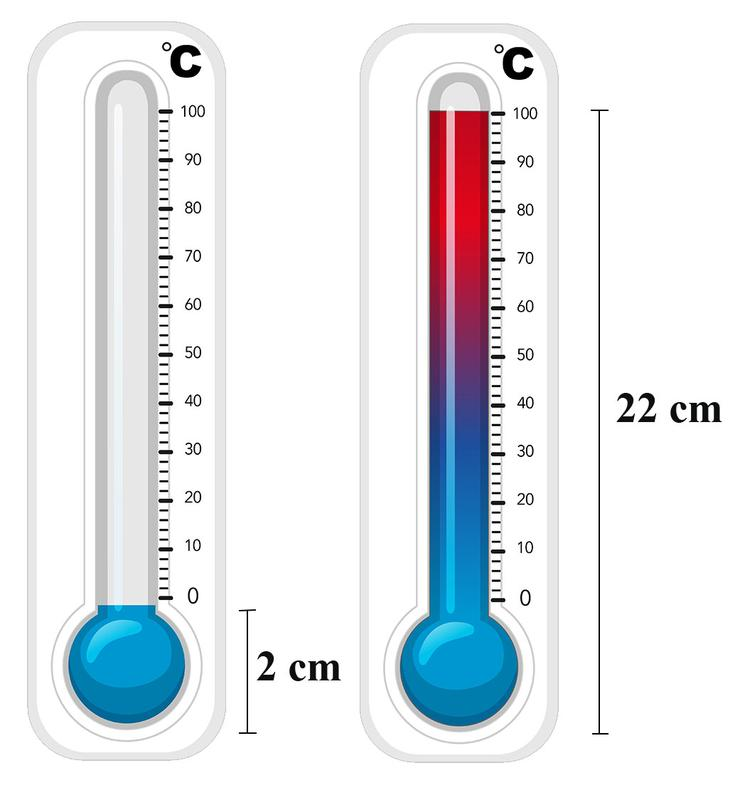
\includegraphics[width=4cm]{Images/nhietke22}}
	\loigiai{
		
		Chiều dài cột thủy ngân tỷ lệ với nhiệt độ. 
		
		Sử dụng phương pháp tỉ lệ để tìm chiều dài tương ứng với một nhiệt độ bất kì.
		
		Xác định chiều dài cột thủy ngân tăng thêm cho mỗi độ Celsius:
		\[ L_{\Delta} = L_{100^\circ C} - L_{0^\circ C} = 22 \, \text{cm} - 2 \, \text{cm} = 20 \, \text{cm} \]
		
		Chiều dài cột thủy ngân tăng thêm tương ứng với một độ Celsius là:
		\[ \Delta L = \dfrac{20 \, \text{cm}}{100^\circ C} = 0.2 \, \text{cm/}^\circ C \]
		
		Nhiệt độ là $50^\circ C$, tức là chiều dài tăng thêm so với lúc $0^\circ C$ sẽ là:
		\[ L_{\text{tăng}} = 50^\circ C \times 0.2 \, \text{cm/}^\circ C = 10 \, \text{cm} \]
		
		Vậy chiều dài cột thủy ngân sẽ là:
		\[ L = L_{0^\circ C} + L_{\text{tăng}} = 2 \, \text{cm} + 10 \, \text{cm} = 12 \, \text{cm} \]
		
	}
	\haidong{4}\end{ex}


\begin{ex} \nguon{3}
	\immini[thm]{Chiều dài của phần thủy ngân trong nhiệt kế là $2\ cm$ ở $0^\circ C$ và $22\ cm$ ở $100^\circ C$. Nhiệt độ là bao nhiêu $^\circ C$ nếu chiều dài của thủy ngân là $8\ cm$?\\
		\shortans[oly]{ } 
		}{
\includegraphics[width=3cm]{images/2024_06_05_4d47cfee1d5b1f81200bg-17}}
	\loigiai{
		
		Ta xét: $\dfrac{\Delta t_{21}}{\Delta \ell_{21}}=\dfrac{t_2 - t_1}{\ell_2 - \ell_1}=\dfrac{100 - 0}{22 - 2}=5^\circ C/cm$
		$\Rightarrow \dfrac{\Delta t}{\Delta \ell}=5^\circ C/cm=$ không đổi
		
		(Khi chiều dài phần thủy ngân tăng thêm $1 cm$ thì nhiệt độ tăng thêm $5^\circ C$)
		
		Ta có: $$\dfrac{\Delta t_{31}}{\Delta \ell_{31}}=\dfrac{t_3 - t_1}{\ell_3 - \ell_1}=\dfrac{t_3 - 0}{8 - 2}=5 \Rightarrow t_3=30^\circ C$$
	}
\end{ex}



\begin{ex} \nguon{4}
	\immini[thm]{Để đo nhiệt độ của các vật thể trong vũ trụ, các nhà vật lí và thiên văn học có thể sử dụng độ biến thiên cường độ bức xạ điện từ phát ra từ một vật. Bước sóng ứng với cường độ lớn nhất được tính theo định luật Wien: $\lambda_{\max}. T=0,2898 \ cm. K$, trong đó $\lambda_{\max}$ là bước sóng với cường độ lớn nhất, $T$ là nhiệt độ của vật tính theo Kelvin. Năm 1965, đỉnh của sóng bức xạ có $\lambda_{\max}=0,107 \ cm$ được phát hiện từ mọi phía của vũ trụ. Nhiệt độ trung bình của vũ trụ là
	\choice
	{\True $-270,3^\circ C$}
	{$270,4^\circ C$}
	{$-70,35^\circ C$}
	{$70,43^\circ C$}}{
\includegraphics[width=3cm]{images/1125}}
	\loigiai{
		Nhiệt độ trung bình vũ trụ theo thang đo nhiệt độ Kelvin:
		$$
		T=\dfrac{0,2898}{\lambda_{\max}}=\dfrac{0,2898}{0,107} \approx 2,7 \ K
		$$
		Nhiệt độ trung bình vũ trụ theo thang đo nhiệt độ Celsius:
		$$
		t=T-273,15=-270,3^\circ C
		$$
	}
\end{ex}
 
\loai{Loại 6: Thang nhiệt độ giả sử}

\begin{ex} \nguon{4}
	Một thang nhiệt độ $Z$ có nhiệt độ đóng băng của nước là $-12^\circ Z$ và khoảng cách mỗi độ chia trong thang đo nhiệt độ $Z$ có độ lớn bằng 0,8 lần khoảng cách mỗi độ chia trong thang đo nhiệt độ Kelvin. Nhiệt độ sôi của nước trong thang nhiệt $Z$ ở áp suất tiêu chuẩn là
	\choice
	{\True $113^\circ Z$}
	{$137^\circ Z$}
	{$68{}^\circ Z$}
	{$92^\circ Z$}\loigiai{
		
		Độ biến thiên $100^\circ C$ tương ứng với độ biến thiên $125^\circ Z$
		
		Nhiệt độ sôi của nước trong thang đo nhiệt độ $Z: t_{Z}=-12+125=113^\circ Z$
	}
\end{ex}


\begin{ex} \nguon{4}
	Một thang đo nhiệt độ $Z$ có nhiệt độ điểm đóng băng của nước là $-15^\circ$ và khoảng cách mỗi độ chia trong thang nhiệt $Z$ có độ lớn gấp 1,6 lần khoảng cách mỗi độ chia trong thang nhiệt Celsius. Nhiệt độ của nước đang sôi trong thang nhiệt $Z$ (áp suất ở điều kiện tiêu chuẩn) là
	\choice
	{$67,5^\circ Z$}
	{$4,5^\circ Z$}
	{$7,5^\circ Z$}
	{\True $47,5^\circ Z$}
	\loigiai{
		
		Gọi $a$ và $b$ lần lượt là khoảng cách mỗi độ chia trong thang đo nhiệt độ $Z$ và thang đo nhiệt độ Celsius, ta có: $a=1,6 b \Rightarrow b=\dfrac{a}{1,6}$
		
		Độ biến thiên nhiệt độ từ điểm đóng băng đến điểm sôi trong thang nhiệt $Z$:
		$$
		\Delta T_{Z}=100b=\dfrac{100}{1,6} a=62,5^\circ Z
		$$
		
		Nhiệt độ sôi của nước theo thang nhiệt $Z$ là: $T_{Z}=-15+62,5=47,5^\circ Z$.
	}
\end{ex}
\loai{DS}
\begin{ex} \nguon{4}
	Biết rằng mối liên hệ giữa các giá trị nhiệt độ trên hai thang đo nhiệt độ là Fahrenheit $t\ (^\circ F)$ và Celsius $t\ (^\circ C)$ được cho bởi công thức $t\ (^\circ F)=32+1,8t\ (^\circ C)$.
	\choiceTF[t]
	{\True Nhiệt độ cơ thể người là $37^\circ C$ tương ứng với $98,6^\circ F$}
	{\True Độ biến thiên nhiệt độ theo hai thang đo nhiệt độ là khác nhau}
	{\True Tại nhiệt độ $-40^\circ C$ thì giá trị nhiệt độ trên hai thang đo là như nhau}
	{Giá trị nhiệt độ khi ghi nhận theo thang đo nhiệt độ Fahrenheit luôn lớn hơn giá trị nhiệt độ ghi nhận theo thang đo nhiệt độ Celsius}
	\loigiai{
		\begin{itemchoice}
			\itemch ĐÚng
			\itemch ĐÚng
			\itemch ĐÚng
			\itemch Sai. Ví dụ $t=-50^\circ C$ thì $t_{F}=-58^\circ F$.
		\end{itemchoice}
	}
\end{ex}
\begin{ex} \nguon{4}
	Dùng một nhiệt kế theo thang đo nhiệt độ Kelvin để đo nhiệt độ của các lò nấu chảy kim loại. Khoảng giá trị nhiệt độ của nhiệt kế có thể đo được từ $400 \ K$ đến $1460 \ K$.
	\choiceTF[t]
	{Biết rằng bạc có nhiệt độ nóng chảy là $960^\circ C$, khi đó nếu dùng nhiệt kế trên thì giá trị trên nhiệt kế là $687 \ K$}
	{Dùng nhiệt kế trên vẫn có thể khảo sát sự tăng nhiệt độ trong quá trình đun sôi nước}
	{\True Nhiệt kế trên có thể sử dụng để đo nhiệt độ khi nấu chảy thiếc có nhiệt độ nóng chảy $232^\circ C$}
	{Nếu nhiệt độ của lò nung thấp hơn $1460^\circ C$ thì nhiệt kế vẫn có thể sử dụng được}
	\loigiai{
		\begin{itemchoice}
			\itemch Sai. Giá trị trên nhiệt kế là $1233 \ K$.
			\itemch Sai. Khoảng giá trị đo của nhiệt kế nằm ngoài khoảng nhiệt độ khi đun nước.
			\itemch Đúng.
			\itemch Sai. Giới hạn trên của nhiệt kế là $1187^\circ C$
		\end{itemchoice}
	}
\end{ex}

